\section{Experiments}
\label{sec:experiments}
We will now consider the certification algorithm and repair algorithm's fairness/utility tradeoff experimentally on three data sets.  The first is the \emph{Ricci data set} at the heart of the Ricci v. DeStefano case \cite{Ricci09}.  It consists of 118 test taker entries, each including information about the firefighter promotion exam taken (Lieutenant or Captain), the score on the oral section of the exam, the written score, the combined score, 
%(weighting the written score at 60\% and the oral score at 40\%), 
and the race of the test taker (black, white, or Hispanic).  In our examination of the protected race attribute, we will group the black and Hispanic test takers into a single non-white category.  The classifier originally used to determine which test takers to promote was the simple threshold classifier that allowed anyone with a combined score of at least 70\% to be eligible for promotion \cite{Miao11RicciStats}.  Although the true number of people promoted was chosen from the eligible pool according to their ranked ordering and the number of slots available, for simplicity in these experiments we will describe all eligible candidates as having been promoted.  We use a random two-thirds / one-third split for the training / test data.

\looseness-1 The other two data sets we will use are from the UCI Machine Learning Repository\footnote{\url{http://archive.ics.ucu.edu/ml}}.  So that we can compare our results to those of Zemel et al. \cite{icml2013_zemel13}, we will use the same data sets and the same decisions about what constitutes a sensitive attribute as they do.  First, we will look at the \emph{German credit} data set, also considered by  Kamiran and Calders \cite{Kamiran09Classifying}.  It contains 1000 instances, each of which consists of 20 attributes and a categorization of that instance as GOOD or BAD.  The protected attribute is Age.  In the examination of this data set with respect to their discriminatory measure, Kamiran and Calders found that the most discrimination was possible when splitting the instances into YOUNG and OLD at age 25 \cite{Kamiran09Classifying}.  We will discretize the data accordingly to examine this potential worst case.  We use a random two-thirds / one-third split for the training / test data.


We also look at the \emph{Adult income} data set, also considered by Kamishima et al. \cite{Kamishima11Fairness}.  It contains 48,842 instances, each of which consists of 14 attributes and a categorization of that person as making more or less than \$50,000 per year.  The protected attribute we will examine is Gender.  Race is also an attribute in the data, and it will be excluded for classification purposes, except for when examining the effects of having multiple protected attributes - in this case, race will be categorized as white and non-white. The training / test split given in the original data is also used for our experiments.

For each of these data sets, we look at a total of 21 versions of the data - the original data set plus 10 partially or fully repaired attribute sets for each of the combinatorial and geometric partial repairs.  These are the repaired attributes for $\lambda \in [0,1]$ at increments of $0.1$.  Data preprocessing was applied before the partial repair algorithm was run.

\vspace*{0.1in}\mypara{Preprocessing.} Datasets were preprocessed as follows:
\begin{enumerate}
\item Remove all protected attributes from $Y$. This ensures that we are not trying to learn a classifier that depends on other protected attributes that might correlate with the target protected attribute.  (The repair process does still get to know $X$.)
\item Remove all unordered categorical features since our repair procedure assumes that the space of values is ordered.  Ordered categories are converted to integers.\footnote{On the Adult Income data, it happens that all missing values were of these unordered categorical columns, so no data sets had missing values after this step.}
\item Scale each feature so that the minimum is zero and the maximum is one.
\end{enumerate}

\vspace*{0.1in}\mypara{Classifiers.} Three different classifiers were used as oracles for measuring discrimination (under the disparate impact measure and a measure by Zemel et al. \cite{icml2013_zemel13}), and to test the accuracy of a classification after repair.  The classifiers used for our experimental tasks were provided by the Scikit-learn\footnote{\url{http://scikit-learn.org}.} python package. 
\begin{itemize}
\item [LR:] Logistic Regression: Liblinear's~\cite{fan2008liblinear} logistic regression algorithm for L2 regularization and logistic loss. The classifier was configured to weight the examples automatically so that classes were weighted equally.
\item [SVM:] Support Vector Machine: Liblinear's~\cite{fan2008liblinear} linear SVM algorithm for L2 regularization and L2 loss. The classifier was configured to weight the examples automatically so that classes were weighted equally.
\item [GNB:] Gaussian Na\"ive Bayes: Scikit-Learn's na\"ive Bayes algorithm with a balanced class prior. 
\end{itemize}

\vspace*{0.1in}\mypara{Parameter selection and cross-validation.}
LR and SVM classifiers were cross-validated using three-fold cross validation and the best parameter based on BER was chosen. 
We cross-validated the parameter controlling the tradeoff between regularization and loss, and $13$ parameters between $10^{-3}$ and $10^3$, with logarithms uniformly spaced, were searched.

\vspace*{0.1in}\mypara{Repair details.}
The repair procedure requires a ranking of each attribute.  The numeric values and ordered categorical attributes were ordered in the natural way and then quantiles were used as the ranks.  Since the repair assumes that there is a point at each quantile value in each protected class, the quantiles were determined in the following way.  For each attribute, the protected class with the smallest number of members was determined.  This size determined how many quantile buckets to create.  The other protected classes were then appropriately divided into the same number of quantile buckets, with the median value in each bucket chosen as a representative value for that quantile.  Each quantile value in the fully repaired version is the median of the representative values for that quantile.  The combinatorial partial repair determines all valid values for an attribute and moves the original data part way to the fully repaired data within this space.  The geometric repair assumes all numeric values are allowed for the partial repair.

\subsection{Certification}
The goal in this section is to experimentally validate our certification algorithm, described in \autoref{sec:certifying-lack-of}.  On each of the data sets described above, we attempt to predict the protected attribute from the remaining attributes.  The resulting \ber is compared to $\di(g)$ where $g: Y \to C$, i.e., the disparate impact value as measured when some classifier attempts to predict the class given the non-protected attributes.  From the underlying data, we can calculate the \ber threshold $\epsilon = 1/2 - \beta / 8$.  Above this threshold, any classifier applied to the data will have disparate impact.  The threshold is chosen conservatively so as to preclude false positives (times when we falsely declare the data to be safe from disparate impact).

\begin{figure}
\begin{center}
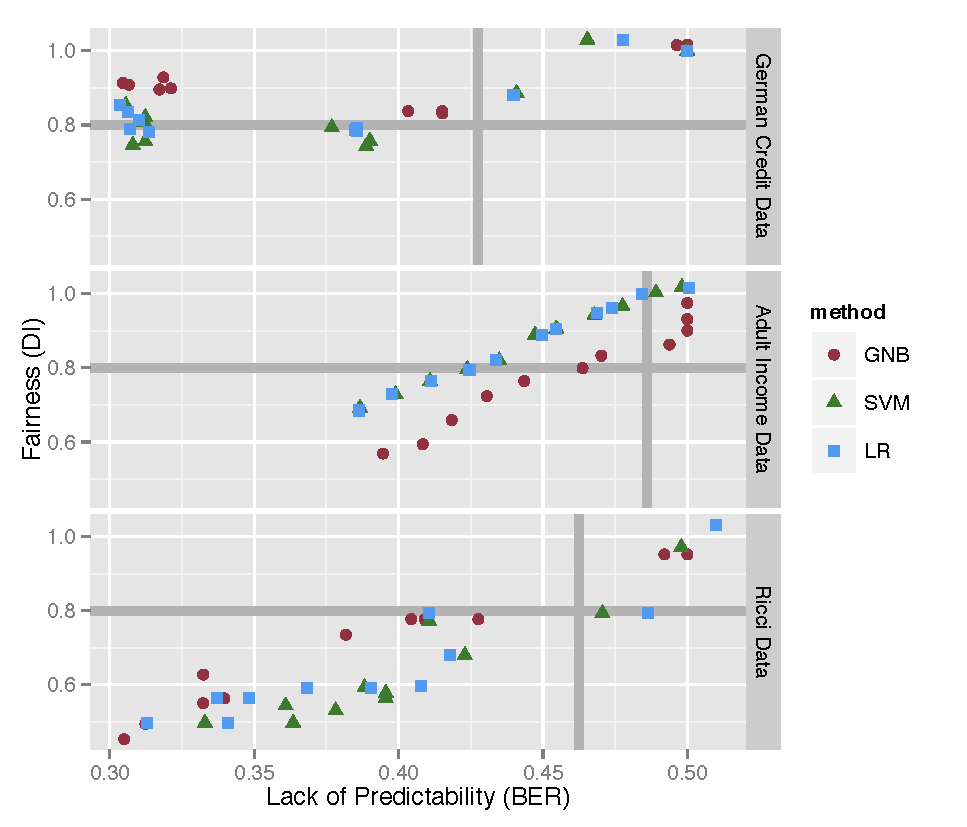
\includegraphics[width=0.75\linewidth]{predictability.pdf}
\caption{Lack of predictability (\ber) of the protected attributes on the German Credit Adult Income, and Ricci data sets as compared to the disparate impact found in the test set when the class is predicted from the non-protected attributes.  The certification algorithm guarantees that points to the right of the \ber threshold are also above $\tau = 0.8$, the threshold for legal disparate impact. For clarity, we only show results using the combinatorial repair, but the geometric repair results follow the same pattern. }
\label{fig:predictability_di}
\end{center}
\end{figure}

\looseness-1 In Figure \ref{fig:predictability_di} we can see that there are no data points greater than the \ber threshold and also much below $\tau = 0.8$, the threshold for legal disparate impact.  The only false positives are a few points very close to the line.  This is likely because the $\beta$ value, as measured from the data, has some error.  We can also see, from the points close to the \ber threshold line on its left but below $\tau$ that while we chose the threshold conservatively, we were not overly conservative.  Still, using a classifier other than the purely biased one in the certification algorithm analysis might allow this threshold to be tightened.

\looseness-1 The points in the upper left quadrant of these charts represent false negatives of our certification algorithm on a specific data set and a specific classifier.  However, our certification algorithm guarantees lack of disparate impact over \emph{any} classifier, so these are not false negatives in the traditional sense.  In fact, when a single data set is considered over all classifiers, we see that all such data sets below the \ber threshold have some classifier that has \di close to or below $\tau = 0.8$.

One seemingly surprising artifact in the charts is the vertical line in the Adult Income data chart at $\ber=0.5$ for the GNB repair.  Recall that the chart is based off of two different confusion matrices - the $\ber$ comes from predicting gender while the disparate impact is calculated when predicting the class.  In a two class system, the $\ber$ cannot be any higher than $0.5$, so while the ability to predict the gender cannot get any worse, the resulting fairness of the class predictions can still improve, thus causing the vertical line in the chart.


\subsection{Fairness / Utility Tradeoff}
\label{sec:fairness_utility}

The goal in this section is to determine how much the partial repair procedure degrades utility.  Using the same data sets as described above, we will examine how the utility (see Definition \ref{def:utility}) changes \di (measuring fairness) increases.  Utility will be defined with respect to the data labels.  Note that this may itself be faulty data, in that the labels may not themselves provide the best possible utility based on the underlying, but perhaps unobservable, desired outcomes.  For example, the results on the test from the Ricci data may not perfectly measure a firefighter's ability and so outcomes based on that test may not correctly predict who should be promoted.  Still, in the absence of knowledge of more precise data, we will use these labels to measure utility.  For the Ricci data, which is unlabeled, we will assume that the true labels are those provided by the simple threshold classifier used on the non-repaired version of the Ricci data, i.e. that anyone with a score of at least 70\% should pass the exam.  Disparate impact (\di) for all data sets is measured with respect to the predicted outcomes on the test set as differentiated by protected attribute.  The SVM described above is used to classify on the Adult Income and German Credit data sets while the Ricci data uses the simple threshold classifier.  The utility ($1-\ber$) shown is based on the confusion matrix of the original labels versus the labels predicted by these classifiers.

\begin{figure}
  \begin{center}
    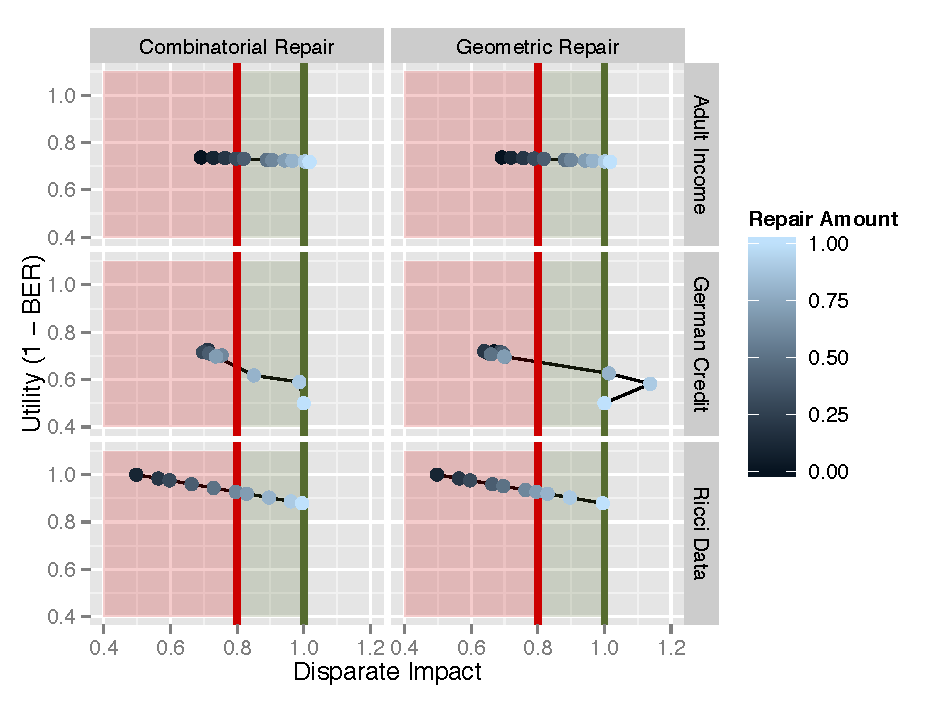
\includegraphics[width=0.75\linewidth]{di_utility_flip.pdf}
    \caption{Disparate impact (\di) vs. utility (1-\ber ) from our combinatorial and geometric partial repair processes using the SVM to classify on the Adult Income and German Credit data sets and the simple threshold classifier on the Ricci data set.  Recall that only points with $\di \geq \tau = 0.8$ are legal.  $\di =1.0$ represents full fairness.}
    \label{fig:fairness_utility}
  \end{center}
\end{figure}

The results, shown in Figure \ref{fig:fairness_utility}, demonstrate the expected decay over utility as fairness increases.  Each unrepaired data set begins with $\di < 0.8$, i.e., it would fail the 80\% rule, and we are able to repair it to a legal value.  For the Adult Income data set, repairing the data fully only results in a utility loss from about 74\% to 72\%, while for the German Credit data, repairing the data fully reduces the utility from about 72\% to 50\% - essentially random.  We suspect that this difference in decay is inherent to the class decisions in the data set (and the next section will show that other existing fairness repairs face this same decay).  We suspect that the lack of linearity in the utility decay in the German Credit data after it has fairness greater than $\di = 0.8$ is due to this low utility.

Looking more closely at the charts, we notice that some of the partially repaired data points have $\di > 1$.  Since \di is calculated with respect to fixed majority and minority classes, this happens when the classifier has given a good outcome to proportionally more minority than majority class members.  These points should be considered unfair to the majority class.

Figure \ref{fig:fairness_utility} also shows that combinatorial and geometric repairs have similar \di and utility values for all partial repair data sets.  This means that either repair can be used.

\looseness-1 \vspace*{0.1in}\mypara{Multiple Protected Attributes.}
Our repair procedure can operate over the joint distribution of multiple protected attributes.  To examine how this affects utility, we considered the Adult Income data set repaired by gender only, race only, and over both gender and race.  
For the repairs with respect to race, a binary racial categorization of white and non-white is used.  Repairs with respect to both race and gender are taken over the joint distribution.  In the joint distribution case, the \di calculated is the average of the \di of each of the three protected sets (white women, non-white men, and non-white women) with respect to the advantaged group (white men).  The classifier used to predict the class from the non-protected attributes is the SVM described earlier.

\begin{figure}
\begin{center}
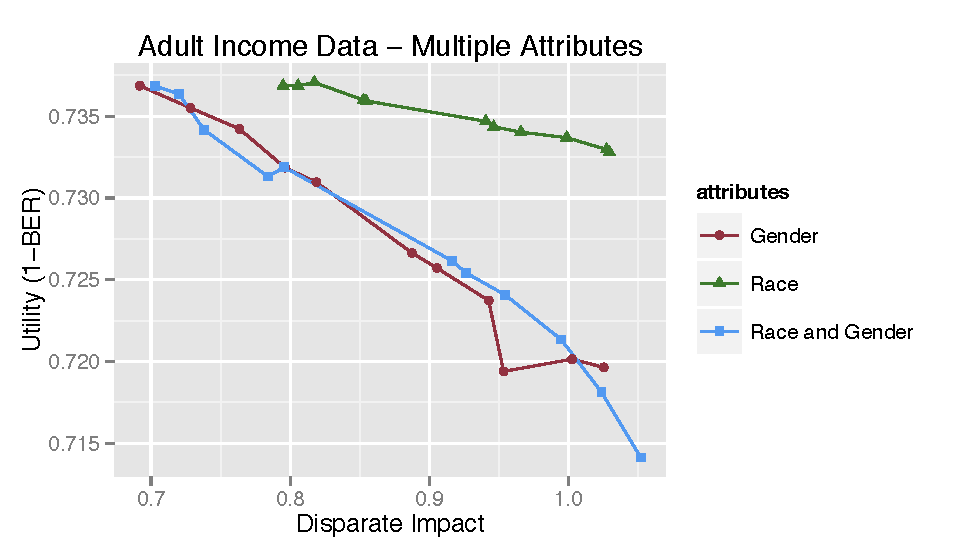
\includegraphics[width=0.75\linewidth]{adult_multiple.pdf}
\caption{Disparate impact (\di) vs. utility (1-\ber ) from our combinatorial and geometric partial repair processes using the SVM as the classifier.  For clarity in the figure, only the combinatorial repairs are shown, though the geometric repairs follow the same pattern.}
\label{fig:fairness_utility_multiple}
\end{center}
\end{figure}

\looseness-1 The results, shown in Figure \ref{fig:fairness_utility_multiple}, show that the utility loss over the joint distribution is close to the maximum of the utility loss over each protected attribute considered on its own.  In other words, the loss does not compound.  These good results are likely due in part to the size of the data set allowing each subgroup to still be large enough.  On such data sets, allowing all protected attributes to be repaired appears reasonable.


\subsection{Comparison to previous work}

Here, we compare our results to related work on the German credit data and Adult income data sets.  Logistic regression is used as a baseline comparison, fair naive Bayes is the solution from Kamiran and Calders \cite{Kamiran09Classifying}, regularized logistic regression is the repair method from Kamishima et al. \cite{Kamishima11Fairness}, and learned fair representations is Zemel et al.'s solution \cite{icml2013_zemel13}.  All comparison data is taken from Zemel et al.'s implementations \cite{icml2013_zemel13}.  Zemel et al. define discrimination as $(1-\alpha) - \beta$.  So that increasing Zemel scores mean that fairness has increased, as is the case with \di, we will look at the \emph{Zemel fairness} score which we define as $1 - ((1-\alpha) - \beta) = 2 \cdot \ber$.  Accuracy is the usual rate of successful classification.  Unlike the compared works, we do not choose a single partial repair point.  Figure \ref{fig:zemel_accuracy} shows our fairness and accuracy results for both combinatorial and geometric partial repairs for values of $\lambda \in [0,1]$ at increments of $0.1$ using all three classifiers described above.

\begin{figure}
  \begin{center}
    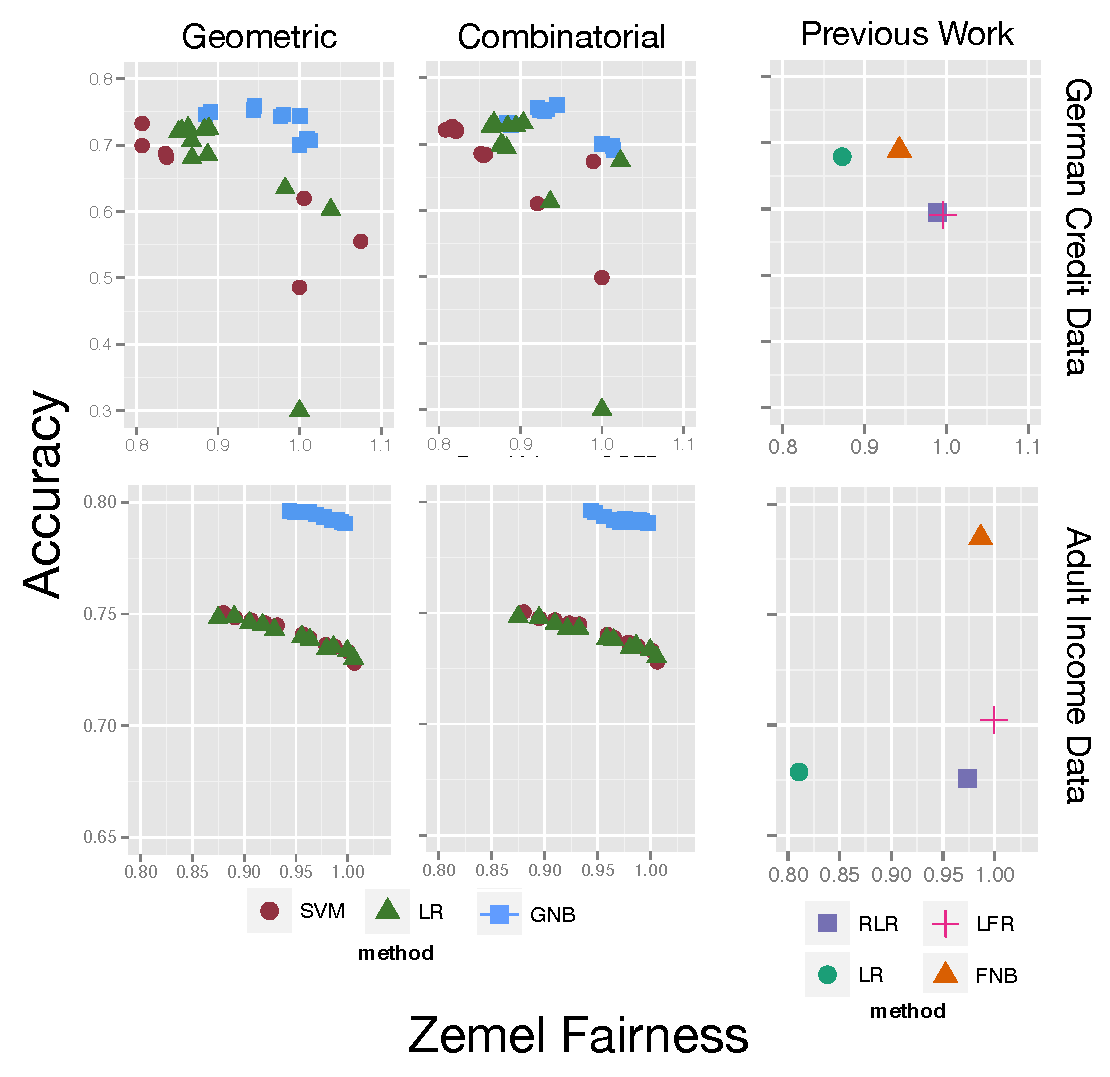
\includegraphics[width=0.75\linewidth]{zemel.pdf}
    \caption{Zemel fairness vs. accuracy from our combinatorial and geometric partial repairs as compared to previous work. Legend: RLR, Regularized Logistic Regression \cite{Kamishima11Fairness}; LFR, Learned Fair Representations \cite{icml2013_zemel13}; FNB, Fair Na\"{i}ve Bayes \cite{Kamiran09Classifying}; GNB, Gaussian Na\"{i}ve Bayes with balanced prior; LR, Logistic Regression; SVM, Support Vector Machine.}
    \label{fig:zemel_accuracy}
  \end{center}
\end{figure}

Figure \ref{fig:zemel_accuracy} shows that our method can be flexible with respect to the chosen classifier.  Since the repair is done over the data, we can choose a classification algorithm appropriate to the data set.  For example, on the Adult Income data set the repairs based on Na\"{i}ve Bayes have better accuracy at high values of fairness than the repairs based on Logistic Regression.  On the German and Adult data sets our results show that for any fairness value a partially repaired data set at that value can be chosen and a classifier applied to achieve accuracy that is better than competing methods.

Since the charts in Figure \ref{fig:zemel_accuracy} include unrepaired data, we can also separate the effects of our classifier choices from the effects of the repair.  In each classifier repair series, the data point with the lowest Zemel fairness (furthest to the left) is the original data.  Comparing the original data point when the LR classifier was used to the LR classifier used by Zemel et al. as a comparison baseline, we see a large jump in both fairness and accuracy.  Configuring the classifier to weight classes equally may have accounted for this improvement.



%%% Local Variables:
%%% mode: latex
%%% TeX-PDF-mode: t
%%% TeX-master: "bias"
%%% End:
